
\section{Pessimisme ou optimisme?}
\label{repl:sec:schemas}

De multiples serveurs, possiblement distants les uns des autres, hébergent une
réplique d'une donnée. Lorsqu'une réplique est modifiée, sa modification est
répercutée sur les autres répliques. Les deux schémas de réplication définissent
la manière dont une modification est acceptée. Cela influe sur les propriétés du
système. En particulier, les dimensions que peuvent atteindre les systèmes, en
nombre de répliques, s'en trouve impactées.

\subsection{Réplication pessimiste}

L'objectif de la réplication pessimiste est simple. Il consiste à donner
l'illusion que la donnée manipulée est unique, indépendemment du nombre de
répliques réel. Ainsi, il devient facile de raisonner sur les données puisque
leurs spécifications sont proches de celles proposées dans un contexte
non-réparti -- sans réplications.

Toutefois, avant qu'une modification ne soit réellement effectuée, il est
nécessaire qu'elles soient validées. L'autorité décisionnelle diffère en fonction
des approches :
\begin{itemize}
\item [\textbf{Autorité centrale~\cite{alsberg1976principle} :}] l'un des
  serveurs est désigné responsable. Ceux qui souhaitent modifier la donnée sont
  alors dans l'obligation de demander l'accès exclusif pendant la mise en place
  de cette modification. Dans l'intervalle, les autres répliques ne peuvent
  soumettre de modifications. Enfin, lorsque la modification est achevée, la
  main est rendue au serveur qui peut autoriser d'autres modifications. On parle
  de verrou (\emph{lock}).
\item [\textbf{Quorum~\cite{gifford1979weighted} :}] un ensemble de serveurs est
  désigné responsable. Chacune des modifications est soumise à un vote quant à
  son acceptation. Au dessus d'un certain seuil de vote positif ou négatif, la
  modification est autorisée ou non.
\end{itemize}


\begin{figure*}
  \centering
  \subfloat[Une demande de modification est effectuée.]
  [Le serveur $n_5$ demande au cœur décisionnel si sa modification est acceptée.]
  {
\begin{tikzpicture}[scale=1.2]

  \newcommand\X{35pt};
  \newcommand\Y{35pt};

  \draw[fill=white, very thick](0*\X, 0*\Y)
  node{$n_1$} +(-5pt,-5pt) rectangle +(5pt,5pt);
  \draw[fill=white, very thick](1*\X,-1*\Y)
  node{$n_2$} +(-5pt,-5pt) rectangle +(5pt,5pt);
  \draw[fill=white, very thick](2*\X, 0*\Y)
  node{$n_3$} +(-5pt,-5pt) rectangle +(5pt,5pt);

  \draw[fill=white](-1.5*\X,0*\Y) node{$n_4$} +(-5pt,-5pt) rectangle +(5pt,5pt);
  \draw[fill=white, thick, draw=darkblue](-1.5*\X,1*\Y)
  node{\DARKBLUE{$n_5$}} +(-5pt,-5pt) rectangle +(5pt,5pt);
  
  \draw[<->] (5+0*\X, 0*\Y) -- (-5+2*\X,0*\Y);
  \draw[<->] (0*\X, -5+0*\Y) -- (-5+1*\X,-1*\Y);
  \draw[<->] (2*\X, -5+0*\Y) -- (5+1*\X ,-1*\Y);

  \scriptsize
  \draw[<->] (5-1.5*\X,0*\Y) -- (-5+0*\X,0*\Y);
  \draw[->, thick, draw=darkblue] (5-1.5*\X, 1*\Y) --
  node[anchor=south west, align=left]
  {\DARKBLUE{ask permission}\\\DARKBLUE{for modification}\\\DARKBLUE{on replica}}
  (-5+0*\X,5+0*\Y);
  
  \draw(1*\X, -0.5*\Y) node[anchor=south, align=center]{decisionnal\\chamber};

  % \scriptsize
  % \draw[->,dashed,very thick, color=darkblue](5+0*\X, 0*\Y) -- 
  % node[anchor=south]{(a)}(-5+ 2*\X, 0*\Y);
  % \draw[->] (-5+2*\X, 5pt) -- (5+\X, \Y);
  % \draw[->] (-5+2*\X, 5pt) --  (5+\X, 2*\Y);
  % \draw[->] (-5+2*\X, -5pt) -- (5+\X, -\Y);
  % \draw[->] (-5+2*\X, -5pt) -- (5+\X, -2*\Y);

  % \normalsize
  % \draw[fill=white, very thick, draw=darkblue]
  % (0*\X, 0*\Y) node{\DARKBLUE{$n_1$}} +(-5pt,-5pt) rectangle +(5pt,5pt);
  % \draw[fill=white, very thick]
  % (2*\X, 0*\Y) node{$n_2$} +(-5pt,-5pt) rectangle +(5pt,5pt);

  % \draw[fill=white](1*\X,2*\Y) node{$n_6$} +(-5pt,-5pt) rectangle +(5pt,5pt);
  % \draw[fill=white](1*\X,1*\Y) node{$n_5$} +(-5pt,-5pt) rectangle +(5pt,5pt);
  % \draw[fill=white](1*\X,-1*\Y) node{$n_4$} +(-5pt,-5pt) rectangle +(5pt,5pt);
  % \draw[fill=white](1*\X,-2*\Y) node{$n_3$} +(-5pt,-5pt) rectangle +(5pt,5pt);
  
\end{tikzpicture}}
  \hspace{40pt}
  \subfloat[Une autre demande est faite pendant que le cœur s'occupe de 
  la première demande.]
  [Le serveur $n_4$ demande également si sa modification est acceptée pendant
  que le cœur est occupé avec la modification de $n_5$.]
  {
\begin{tikzpicture}[scale=1.2]

  \newcommand\X{35pt};
  \newcommand\Y{35pt};

  \draw[fill=white, very thick](0*\X, 0*\Y)
  node{$n_1$} +(-5pt,-5pt) rectangle +(5pt,5pt);
  \draw[fill=white, very thick](1*\X,-1*\Y)
  node{$n_2$} +(-5pt,-5pt) rectangle +(5pt,5pt);
  \draw[fill=white, very thick](2*\X, 0*\Y)
  node{$n_3$} +(-5pt,-5pt) rectangle +(5pt,5pt);

  \draw[fill=white, thick, draw=darkblue](-1.5*\X,0*\Y)
  node{\DARKBLUE{$n_4$}} +(-5pt,-5pt) rectangle +(5pt,5pt);
  \draw[fill=white](-1.5*\X,1*\Y) node{$n_5$} +(-5pt,-5pt) rectangle +(5pt,5pt);

  \scriptsize  
  \draw[<-, thick, draw=darkblue] (5+0*\X, 0*\Y) --
  node[anchor=south]{\DARKBLUE{Ok. Ok?}} (-5+2*\X,0*\Y);
  \draw[->, thick, draw=darkblue] (0*\X, -5+0*\Y) --
  node[anchor=east]{\DARKBLUE{Ok. Ok?}}  (-5+1*\X,-1*\Y);
  \draw[<-, thick, draw=darkblue] (2*\X, -5+0*\Y) --
  node[anchor=west]{\DARKBLUE{Ok. Ok?}} (5+1*\X ,-1*\Y);


  \draw[->, draw=darkblue] (5-1.5*\X,0*\Y) --
  node[anchor=north]{\DARKBLUE{ask permission}}
  (-5+0*\X,0*\Y);
  \draw[<->] (5-1.5*\X, 1*\Y) -- node[anchor=south west]{wait}
  (-5+0*\X,5+0*\Y);
  
  \draw(1*\X, -0.5*\Y) node[anchor=south, align=center]{decisionnal\\chamber};

  % \scriptsize
  % \draw[->,dashed,very thick, color=darkblue](5+0*\X, 0*\Y) -- 
  % node[anchor=south]{(a)}(-5+ 2*\X, 0*\Y);
  % \draw[->] (-5+2*\X, 5pt) -- (5+\X, \Y);
  % \draw[->] (-5+2*\X, 5pt) --  (5+\X, 2*\Y);
  % \draw[->] (-5+2*\X, -5pt) -- (5+\X, -\Y);
  % \draw[->] (-5+2*\X, -5pt) -- (5+\X, -2*\Y);

  % \normalsize
  % \draw[fill=white, very thick, draw=darkblue]
  % (0*\X, 0*\Y) node{\DARKBLUE{$n_1$}} +(-5pt,-5pt) rectangle +(5pt,5pt);
  % \draw[fill=white, very thick]
  % (2*\X, 0*\Y) node{$n_2$} +(-5pt,-5pt) rectangle +(5pt,5pt);

  % \draw[fill=white](1*\X,2*\Y) node{$n_6$} +(-5pt,-5pt) rectangle +(5pt,5pt);
  % \draw[fill=white](1*\X,1*\Y) node{$n_5$} +(-5pt,-5pt) rectangle +(5pt,5pt);
  % \draw[fill=white](1*\X,-1*\Y) node{$n_4$} +(-5pt,-5pt) rectangle +(5pt,5pt);
  % \draw[fill=white](1*\X,-2*\Y) node{$n_3$} +(-5pt,-5pt) rectangle +(5pt,5pt);
  
\end{tikzpicture}}
  \hspace{10pt}
  \subfloat[Une modification est acceptée pendant que l'autre est refusée]
  [La modification de $n_5$ est acceptée tandis que celle de $n_4$ 
  est refusée.]
  {
\begin{tikzpicture}[scale=1.2]

  \newcommand\X{35pt};
  \newcommand\Y{35pt};

  \draw[fill=white, very thick](0*\X, 0*\Y)
  node{$n_1$} +(-5pt,-5pt) rectangle +(5pt,5pt);
  \draw[fill=white, very thick](1*\X,-1*\Y)
  node{$n_2$} +(-5pt,-5pt) rectangle +(5pt,5pt);
  \draw[fill=white, very thick](2*\X, 0*\Y)
  node{$n_3$} +(-5pt,-5pt) rectangle +(5pt,5pt);

  \draw[fill=white](-1.5*\X,0*\Y) node{$n_4$} +(-5pt,-5pt) rectangle +(5pt,5pt);
  \draw[fill=white](-1.5*\X,1*\Y)
  node{$n_5$} +(-5pt,-5pt) rectangle +(5pt,5pt);
  
  \draw[<->] (5+0*\X, 0*\Y) -- (-5+2*\X,0*\Y);
  \draw[<->] (0*\X, -5+0*\Y) -- (-5+1*\X,-1*\Y);
  \draw[<->] (2*\X, -5+0*\Y) -- (5+1*\X ,-1*\Y);

  \scriptsize
  \draw[<-, thick, draw=darkblue] (5-1.5*\X,0*\Y) --
  node[anchor=north]{\DARKBLUE{denied}}(-5+0*\X,0*\Y);
  \draw[<-, thick, draw=darkblue] (5-1.5*\X, 1*\Y) --
  node[anchor=south west]{\DARKBLUE{accepted}}(-5+0*\X,5+0*\Y);
  
  \draw(1*\X, -0.5*\Y) node[anchor=south, align=center]{decisionnal\\chamber};

  % \scriptsize
  % \draw[->,dashed,very thick, color=darkblue](5+0*\X, 0*\Y) -- 
  % node[anchor=south]{(a)}(-5+ 2*\X, 0*\Y);
  % \draw[->] (-5+2*\X, 5pt) -- (5+\X, \Y);
  % \draw[->] (-5+2*\X, 5pt) --  (5+\X, 2*\Y);
  % \draw[->] (-5+2*\X, -5pt) -- (5+\X, -\Y);
  % \draw[->] (-5+2*\X, -5pt) -- (5+\X, -2*\Y);

  % \normalsize
  % \draw[fill=white, very thick, draw=darkblue]
  % (0*\X, 0*\Y) node{\DARKBLUE{$n_1$}} +(-5pt,-5pt) rectangle +(5pt,5pt);
  % \draw[fill=white, very thick]
  % (2*\X, 0*\Y) node{$n_2$} +(-5pt,-5pt) rectangle +(5pt,5pt);

  % \draw[fill=white](1*\X,2*\Y) node{$n_6$} +(-5pt,-5pt) rectangle +(5pt,5pt);
  % \draw[fill=white](1*\X,1*\Y) node{$n_5$} +(-5pt,-5pt) rectangle +(5pt,5pt);
  % \draw[fill=white](1*\X,-1*\Y) node{$n_4$} +(-5pt,-5pt) rectangle +(5pt,5pt);
  % \draw[fill=white](1*\X,-2*\Y) node{$n_3$} +(-5pt,-5pt) rectangle +(5pt,5pt);
  
\end{tikzpicture}}
  \caption{\label{repl:fig:pessimisticexample} Exemple de quorum en réplication
    pessimiste. La modification de $n_5$ est propagée.}
\end{figure*}

La figure~\ref{repl:fig:pessimisticexample} montre un exemple de réplication
pessimiste où le cœur décisionnel est composé de 3 serveurs
$\{n_1,\, n_2,\, n_3\}$ devant unanimement approuver une modification avant
qu'elle soit propagée. Ainsi, le serveur $n_5$ propose une modification des
répliques au cœur décisionnel via $n_1$. Ce dernier l'accepte et transmet la
demande à $n_2$, qui l'accepte et la transmet à son tour à $n_3$, qui l'accepte
et termine la boucle en transmettant à $n_1$.  Dans l'intervalle, $n_4$ propose
une autre modification. La proposition de $n_5$ est acceptée et propagée tandis
que celle de $n_4$ est refusée. Une fois que $n_4$ a réçu les modifications de
$n_5$, il peut retenter de transmettre sa modification s'l la juge toujours
d'actualité. Cet exemple illustre le caractère chronophage du processus : le
vote prend du temps et peut échouer. De plus, si l'un des serveurs du cœur
défaillit, le vote peut échouer alors même que la modification est valide.

La réplication pessimiste est possible lorsque le nombre de répliques est connu,
plutôt petit, et souvent accessible. Ces contraintes sont notamment
satisfaisable dans le Nuage~\cite{mell2011national}. Les répliques proposent
d'avantage de garanties quant aux résultats de la manipulation des
données. Toutefois, de telles guaranties ne sont pas toujours nécéssaires et
leur coût élévé n'est plus justifié. La réplication optimiste constitue alors
une alternative possible.

\subsection{Réplication optimiste}

En 1987, Demers et al. décrivent une base de données répliquée sur plusieurs
centaines de machines pouvant communiquer entre elles au travers de materiels
aux capacités hétérogènes~\cite{demers1987epidemic}. Du fait de ces dimensions,
la réplication pessimiste semble impossible.

La réplication optimiste~\cite{johnson1975maintenance, saito2005optimistic} est
un paradigme de réplication consistant à appliquer les modifications directement
sur la réplique locale.  Ainsi, les données sont toujours disponibles et
réactives aux changements effectués. Ensuite, les modifications sont disséminées
aux autres serveurs hébergeant une réplique où elles sont appliquées. Au
contraire des approches pessimistes, les approches optimistes ne vérouillent pas
les données lors des changements. En revanche, le critère de cohérence assuré
est plus faible. En particulier, les répliques ont l'autorisation d'avoir des
états temporairement divergeant entre eux :

\begin{itemize}
\item [\textbf{Cohérence à terme~\cite{bailis2013eventual} :}] lorsque toutes
  les modifications ont été reçues et appliquées par toutes les répliques,
  celle-ci possèdent un état équivalent.

  Puisque ``\emph{toutes} les modifications'' constitue un ensemble peu réaliste
  pour raisonner sur une exécution réelle, un définition plus précise porte sur
  un sous-ensemble de ces modifications :
\item [\textbf{Cohérence forte à terme~\cite{shapiro2011conflict} :}] les
  répliques ayant réçu et appliqué les mêmes modifications possèdent un état
  équivalent.
\end{itemize}

\begin{figure*}
  \centering
  \subfloat[Modifications concurrentes.]
  [Les serveurs $n_1$ et $n_3$ modifient leur couleur en même temps.]
  {
\begin{tikzpicture}[scale=1.2]

  \newcommand\X{35pt};
  \newcommand\Y{35pt};

  \draw[fill=white, very thick](0*\X, 0*\Y)
  node{$n_1$} +(-5pt,-5pt) rectangle +(5pt,5pt);
  \draw[fill=white, very thick](1*\X,-1*\Y)
  node{$n_2$} +(-5pt,-5pt) rectangle +(5pt,5pt);
  \draw[fill=white, very thick](2*\X, 0*\Y)
  node{$n_3$} +(-5pt,-5pt) rectangle +(5pt,5pt);

  \draw[<-] (5+0*\X, -3+0*\Y) -- (-5+2*\X, -3+*\Y);
  \draw[->] (5+0*\X,  3+0*\Y)  -- (-5+2*\X, 3+*\Y);

  \draw[<-] (-3+0*\X, -5+0*\Y) -- (-5+1*\X,-3-1*\Y);
  \draw[->] ( 3+0*\X, -5+0*\Y) -- (-5+1*\X, 3-1*\Y);

  \draw[<-] (-3+2*\X, -5+0*\Y) -- (5+1*\X ,-3-1*\Y);
  \draw[->] ( 3+2*\X, -5+0*\Y) -- (5+1*\X ,3-1*\Y);

  % \scriptsize
  % \draw[->,dashed,very thick, color=darkblue](5+0*\X, 0*\Y) -- 
  % node[anchor=south]{(a)}(-5+ 2*\X, 0*\Y);
  % \draw[->] (-5+2*\X, 5pt) -- (5+\X, \Y);
  % \draw[->] (-5+2*\X, 5pt) --  (5+\X, 2*\Y);
  % \draw[->] (-5+2*\X, -5pt) -- (5+\X, -\Y);
  % \draw[->] (-5+2*\X, -5pt) -- (5+\X, -2*\Y);

  % \normalsize
  % \draw[fill=white, very thick, draw=darkblue]
  % (0*\X, 0*\Y) node{\DARKBLUE{$n_1$}} +(-5pt,-5pt) rectangle +(5pt,5pt);
  % \draw[fill=white, very thick]
  % (2*\X, 0*\Y) node{$n_2$} +(-5pt,-5pt) rectangle +(5pt,5pt);

  % \draw[fill=white](1*\X,2*\Y) node{$n_6$} +(-5pt,-5pt) rectangle +(5pt,5pt);
  % \draw[fill=white](1*\X,1*\Y) node{$n_5$} +(-5pt,-5pt) rectangle +(5pt,5pt);
  % \draw[fill=white](1*\X,-1*\Y) node{$n_4$} +(-5pt,-5pt) rectangle +(5pt,5pt);
  % \draw[fill=white](1*\X,-2*\Y) node{$n_3$} +(-5pt,-5pt) rectangle +(5pt,5pt);
  
\end{tikzpicture}}
  \hspace{10pt}
  \subfloat[Plusieurs états possibles.]
  [Les répliques convergent. Plusieurs états de convergence sont possibles.]
  {
\begin{tikzpicture}[scale=1.2]

  \newcommand\X{35pt};
  \newcommand\Y{40pt};
  
  \begin{scope}[shift={(0*\X, 0*\Y)}]
    \draw[fill=darkblue, very thick](0*\X, 0*\Y)
    node{$n_1$} +(-5pt,-5pt) rectangle +(5pt,5pt);
    \draw[fill=darkblue, very thick](1*\X,-1*\Y)
    node{$n_2$} +(-5pt,-5pt) rectangle +(5pt,5pt);
    \draw[fill=darkblue, very thick](2*\X, 0*\Y)
    node{$n_3$} +(-5pt,-5pt) rectangle +(5pt,5pt);
    

    \draw[<->] (5+0*\X, 0*\Y) -- (-5+2*\X, 0*\Y);
    \draw[<->] (0*\X, -5+0*\Y) -- (-5+1*\X, -1*\Y);
    \draw[<->] (2*\X, -5+0*\Y) -- ( 5+1*\X, -1*\Y);
    \scriptsize
    \draw (1*\X, -1.3*\Y)node{(i) blue wins};
  \end{scope}

  \begin{scope}[shift={(3*\X, 0*\Y)}]
    \draw[fill=white, very thick](0*\X, 0*\Y)
    node{$n_1$} +(-5pt,-5pt) rectangle +(5pt,5pt);
    \draw[fill=white, very thick](1*\X,-1*\Y)
    node{$n_2$} +(-5pt,-5pt) rectangle +(5pt,5pt);
    \draw[fill=white, very thick](2*\X, 0*\Y)
    node{$n_3$} +(-5pt,-5pt) rectangle +(5pt,5pt);
        
    \draw[<->] (5+0*\X, 0*\Y) -- (-5+2*\X, 0*\Y);
    \draw[<->] (0*\X, -5+0*\Y) -- (-5+1*\X, -1*\Y);
    \draw[<->] (2*\X, -5+0*\Y) -- ( 5+1*\X, -1*\Y);
    \scriptsize
    \draw (1*\X, -1.3*\Y)node{(ii) white wins};    
  \end{scope}

  \begin{scope}[shift={(0*\X, -2*\Y)}]
    \draw[fill=blue, very thick](0*\X, 0*\Y)
    node{$n_1$} +(-5pt,-5pt) rectangle +(5pt,5pt);
    \draw[fill=blue, very thick](1*\X,-1*\Y)
    node{$n_2$} +(-5pt,-5pt) rectangle +(5pt,5pt);
    \draw[fill=blue, very thick](2*\X, 0*\Y)
    node{$n_3$} +(-5pt,-5pt) rectangle +(5pt,5pt);
    
    \draw[<->] (5+0*\X, 0*\Y) -- (-5+2*\X, 0*\Y);
    \draw[<->] (0*\X, -5+0*\Y) -- (-5+1*\X, -1*\Y);
    \draw[<->] (2*\X, -5+0*\Y) -- ( 5+1*\X, -1*\Y);
    \scriptsize
    \draw (1*\X, -1.3*\Y)node{(iii) both win};    
  \end{scope}

  \begin{scope}[shift={(3*\X, -2*\Y)}]
    \draw[fill=black, very thick](0*\X, 0*\Y)
    node{$n_1$} +(-5pt,-5pt) rectangle +(5pt,5pt);
    \draw[fill=black, very thick](1*\X,-1*\Y)
    node{$n_2$} +(-5pt,-5pt) rectangle +(5pt,5pt);
    \draw[fill=black, very thick](2*\X, 0*\Y)
    node{$n_3$} +(-5pt,-5pt) rectangle +(5pt,5pt);
    
    \draw[<->] (5+0*\X, 0*\Y) -- (-5+2*\X, 0*\Y);
    \draw[<->] (0*\X, -5+0*\Y) -- (-5+1*\X, -1*\Y);
    \draw[<->] (2*\X, -5+0*\Y) -- ( 5+1*\X, -1*\Y);
    \scriptsize
    \draw (1*\X, -1.3*\Y)node{(iv) arbitrary yet convergent value};
  \end{scope}

  
\end{tikzpicture}}
  \caption{\label{repl:fig:optimisticexample} Exemple de réplication optimiste
    avec modifications concurrentes.}
\end{figure*}


Ces critères de cohérence posent de nombreux problèmes par leur manque
d'expressivité. En particulier, l'état équivalent vers lequel les répliques
convergent n'est pas spécifié. Celui-ci peut n'avoir aucun lien avec l'éxecution
souhaitée par l'utilisateur. Par exemple, un ensemble dont l'ajout d'éléments
n'a aucun effet converge vers l'ensemble vide. Bien que d'une complète
inutilité, il maintient la cohérence forte à terme.

Récemment, de nombreux efforts ont été fournis afin de proposer des bases de
données avec cohérence à terme (\REF), ainsi que des langages sur lesquels
raisonner (\REF).

% \begin{figure}
%   \centering
%   
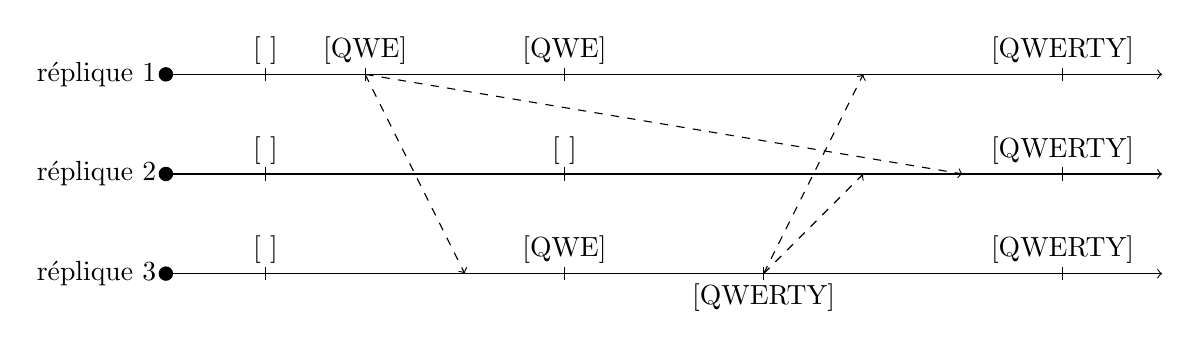
\begin{tikzpicture}[scale=1.2]

  \newcommand\X{30pt};
  \newcommand\Y{30pt};
  
  \draw[->](0pt,   0pt)--(10*\X,   0pt);
  \draw[->](0pt, -1*\Y)--(10*\X, -1*\Y);
  \draw[->](0pt, -2*\Y)--(10*\X, -2*\Y);
  
  \draw[fill=black](0pt, 0pt) node[anchor=east]{réplique 1 }circle(2pt);
  \draw[fill=black](0pt, -1*\Y) node[anchor=east]{réplique 2 }circle(2pt);
  \draw[fill=black](0pt, -2*\Y) node[anchor=east]{réplique 3 }circle(2pt);

  \draw(\X,2pt)--node[anchor=south]{[ ]}( \X,   -2pt);
  \draw(\X,2 -1*\Y)--node[anchor=south]{[ ]}(\X,-2 -1*\Y);
  \draw(\X,2 -2*\Y)--node[anchor=south]{[ ]}(\X,-2 -2*\Y);

  \draw(2* \X,2pt)--node[anchor=south]{[QWE]}(2* \X,   -2pt);
%  \draw(2* \X,2 -1*\Y)--node[anchor=south]{[ ]}(2* \X,-2 -1*\Y);
%  \draw(2* \X,2 -2*\Y)--node[anchor=south]{[ ]}(2* \X,-2 -2*\Y);

  \draw[->, dashed] (2*\X, 0pt) -- (8*\X, -1*\Y);
  \draw[->, dashed] (2*\X, 0pt) -- (3*\X, -2*\Y);

  \draw(4*\X, 2 -0*\Y)--node[anchor=south]{[QWE]}(4*\X,-2 -0*\Y);
  \draw(4*\X, 2 -1*\Y)--node[anchor=south]{[ ]}(4*\X,-2 -1*\Y);
  \draw(4*\X, 2 -2*\Y)--node[anchor=south]{[QWE]}(4*\X,-2 -2*\Y);


  \draw(6*\X, 2 -2*\Y)--node[anchor=north]{[QWERTY]}(6*\X,-2 -2*\Y);


  \draw[->, dashed] (6*\X, -2*\Y)--(7*\X, -0*\Y);
  \draw[->, dashed] (6*\X, -2*\Y)--(7*\X, -1*\Y);

  \draw(9*\X, 2 -0*\Y)--node[anchor=south]{[\BLUE{QWERTY}]}(9*\X,-2 -0*\Y);
  \draw(9*\X, 2 -1*\Y)--node[anchor=south]{[\BLUE{QWERTY}]}(9*\X,-2 -1*\Y);
  \draw(9*\X, 2 -2*\Y)--node[anchor=south]{[\BLUE{QWERTY}]}(9*\X,-2 -2*\Y);


%%  \draw[fill=white, very thick]
%%  (0*\X, 0*\Y) node{$p_1$} +(-5pt,-5pt) rectangle +(5pt,5pt);
%%  \draw[->](-5+\X, 5+2*\Y)to[out=120,in=30](0pt,5+2*\Y); %% 6 -> 7
\end{tikzpicture}
%   \caption{\label{repl:fig:eventualconsistencyexample} Exemple d'éxecution d'un protocole
%     de réplication optimiste dont les répliques convergent vers la séquence
%     'QWERTY'.}
% \end{figure}

% La figure~\ref{repl:fig:eventualconsistencyexample} présente un cas de séquence
% répliquée.  Il existe trois copies d'une séquence initialement vide. La première
% copie insère 'QWE' et en dissémine l'information. La troisième copie reçoit
% l'opération et l'applique localement. Cette copie insère 'RTY' à la suite de
% 'QWE' afin d'obtenir 'QWERTY' et envoie l'information aux deux autres
% copies. Quel que soit l'ordre de réception, le protocole garanti que les copies
% convergent vers un état identique, ici, la séquence 'QWERTY'.


%%% Local Variables:
%%% mode: latex
%%% TeX-master: "../../paper"
%%% End:
